\chapter{Analýza}
\section{Funkční specifikace}
V rámci této práce je zpracován framework ve dvou verzích, pro mobilní platformu Android a mobilní platformu Windows Phone. Řešení musí umožňovat jednoduše vytvářet dva typy komponent, formulář, který umožní uživatelský vstup, a list pro zobrazení většího množství dat uživateli. Kromě vytvoření komponent je nutné poskytnout další funkce, které umožní práci s vytvořenými komponentami, jako je například odeslání dat z komponenty na server. Framework musí samozřejmě disponovat funkcionalitou, která umožní správné vytvoření a nastavení komponenty z hlediska zabezpečení, získávání dat a jejich vložení do komponenty, vzhledu komponenty či její lokalizace. Všechny funkční požadavky jsou uvedeny v následujícím seznamu položek.
\subsection{Funkční požadavky}
\begin{itemize}
\item Framework bude umožňovat automaticky vytvořit formulář nebo list na základě dat získaných ze serveru.
\item Framework bude umožňovat získat ze serveru data, kterými komponentu naplní.
\item Framework bude umožňovat naplnit formulář i list daty.
\item Framework bude umožňovat odeslat data z formuláře zpět na server.
\item Framework bude umožňovat používat lokalizační texty.
\item Framework bude umožňovat validaci vstupních dat na základě definice komponenty, kterou obdržel ze serveru.
\item Framework bude umožňovat upravit vzhled komponenty pomocí skinů.
\item Framework bude umožňovat koncovému uživateli specifikovat zdroje definic komponent, dat a cíle pro jejich odeslání ve formátu XML.
\item Framework bude umožňovat vytvářet následující formulářová pole - textová, číselná, pole pro hesla, pro datum, dropdown pole, checkboxy, option buttony.
\item Framework bude umožňovat resetovat úpravy ve formuláři nebo formulář vyčistit.
\item Framework bude umožňovat získat data z formuláře i listu.
\item Framework bude umožňovat zneviditelnit chyby, které se uživateli zobrazí při neúspěšné validaci formuláře.
\item Framework bude umožňovat jednoduše získat komponentu i na jiném místě v programu, než kde ji vytvořil.
\item Framework bude umožňovat generování komponent určených pouze pro čtení.
\end{itemize}

Pro uživatele, který bude framework využívat, bude proces tvorby komponenty zapouzdřen. Nemusí znát strukturu definice komponenty, ani jak se komponenta tvoří či naplňuje daty. Bude potřebovat znát jen kód pro vytvoření komponenty, akce, které lze nad komponentou provádět a jak specifikovat, odkud se bere definice komponenty, data pro její naplnění a kam se případně data odešlou.

\section{Popis architektury a komunikace}
\subsection{Definice komponent}
Frameworky pro mobilní platformy Android a Windows Phone, které je cílem vytvořit, navazují, jak už bylo zmíněno, na projekt AFSwinx a AFRest \cite{tomasek-thesis}. Tento framework vytváří na straně serveru tzv. definice komponent, které komponentu popisují z hlediska vzhledu, rozložení i obsahu. Jedná se tedy o metadata \cite{metadata}, neboli data, která popisují další data. Taková definice vzniká na serveru ve formátu XML na základě inspekce modelu, kterou zprostředkovává knihovna AspectFaces a AFRest ji zobecňuje a převádí do formátu JSON. Na serveru zastupuje roli modelu databázová entita a vlastnosti, které má inspekce modelu zachytit a do definice promítnout, jsou určeny datovými typy atributů a pomocí anotací.
Definice komponenty, kterou lze získat ze serveru, obsahuje tyto infomace:
\begin{itemize}
\item název definice
\item celkové rozložení komponenty
\item informace o polích v daném pořadí, které se mají v komponentě vyskytnout
\end{itemize}
V informacích o poli lze nalézt:
\begin{itemize}
\item typ widgetu, kterým má být vytvářené pole reprezentováno
\item jednoznačný identifikátor v rámci komponenty
\item popisek neboli label
\item viditelnost
\item zda má být pole určeno jen pro čtení
\item zda se jedná o primitivní či složený datový typ
\item validační pravidla
\item v případě některých widgetů i možnosti, ze kterých si má uživatel vybírat
\end{itemize}

Cílem autora AFSwinx a AFRest \cite{tomasek-thesis} bylo, aby tyto definice komponent byly nezávislé na platformě, což se i jejich využitím na mobilních platformách potvrzuje. Se strukturou těchto definic oba frameworky počítají, na základě tohoto formátu se definice na klientovi udržuje a z ní tvoří uživatelské rozhraní. 

\subsection{Získání definice ze serveru}
Definici komponenty je možné získat pomocí HTTP dotazu na konkrétní zdroj na serveru, který je schopen takovou definici za použití AFSwinx a AFRest poskytnout \cite{tomasek-thesis}. Tento konkrétní zdroj poskytující definici komponenty je nutné specifikovat. Také lze určit dva další zdroje - zdroj dat a zdroj, na který se má odeslat uživatelský vstup. Frameworky mají, dle požadavků výše, umožňovat uživateli tyto zdroje specifikovat ve formátu XML. Již v AFSwinx a AFRest byl pro tento účel vytvořen XML soubor a k němu příslušný XML parser, které je v Android verzi frameworku žádoucí z hlediska efektivity využít. Jelikož je AFSwinx a AFRest napsaný v Javě a Windows Phone nepodporuje Javu, nýbrž jazyk C\#, a tedy ani import JAR souborů, nelze parser znovu použít i ve Windows Phone frameworku a je nutné ho přepsat. Část z kódu popisující zdroj pro metadata je zobrazen v následujícím úryvku kódu \ref{code:xmlSourceShort} ze zmíněného XML souboru. Celý kód tohoto připojení, který obsahuje také popis zdrojů pro data a odeslání formuláře, lze nalézt v příloze \ref{code:xmlSource}. 

\begin{lstlisting}[caption=Ukázka XML specifikace zdroje pro metadata,
label={code:xmlSourceShort}, basicstyle=\footnotesize]
<?xml version="1.0" encoding="UTF-8"?>
<connectionRoot xmlns:xsi="http://www.w3.org/2001/XMLSchema-instance">
   <connection id="personProfile">
      <metaModel>
         <endPoint>toms-cz.com</endPoint>
         <endPointParameters>/AFServer/rest/users/profile</endPointParameters>
         <protocol>http</protocol>
         <port></port>
         <header-param>
            <param>content-type</param>
            <value>Application/Json</value>
         </header-param>
      </metaModel>
   </connection>
</connectionRoot>
\end{lstlisting}

Z ukázky \ref{code:xmlSource} plyne, že jsou zdroje nadefinovány URL adresou rozdělenou na části a dodatečnými parametry, jako je forma dat, která lze očekávat, nebo zabezpečení. Například definice profilového formuláře se nachází na adrese \url{http://toms-cz.com/AFServer/rest/users/profile} a je očekávána ve formátu JSON, což je nadefinováno pomocí parametru content-type. Pokud by byl specifikován port, přibude za toms-cz.com dvojtečka a jeho hodnota. Zdroj dat je nadefinován v uzlu <data> a zdroj, na který se odešle uživatelský vstup, určuje uzel <send>. Lze také specifikovat metodu (get, post, put, delete), která se pro kontaktování zdroje použije. Pro data a metamodel je v základu použita metoda GET a pro odeslání metoda POST. V případě, že je přístup ke zdroji zabezpečen, je použita autorizace typu basic.

Výrazy ve složených závorkách označené vpředu pomocí znaku \# jsou určeny k nahrazení hodnotou. V AFSwinx a AFRest \cite{tomasek-thesis} se klíč ve složených závorkách hledá v mapě parametrů pro připojení, kterou framework předává jako argument metodě kontaktující zdroj, a nahrazuje se hodnotou v ní pod klíčem uloženou. Umožňuje to tak nadefinovat zdroj v XML souboru pouze jednou, například pro více různých uživatelů. Klíč a hodnotu si může uživatel nastavit sám, důležité však je, aby se shodovaly klíče ve zmíněné mapě a v souboru. V zájmu znovupoužití XML souboru a parseru se tedy tomuto chování oba tvořené frameworky přizpůsobují.

\subsection{Reprezentace metadat ve frameworku}
Získaná metadata je potřeba ve frameworku udržovat. AFSwinx už pro to určitou strukturu definuje \cite{tomasek-thesis} a je tedy žádoucí ji opětovně využít. Tuto část systému, která uchová získané informace o komponentě, zachycuje následující doménový model, vytvořený za pomocí UML. Unified Modeling Language (UML) \cite{UmlArlow} je univerzální jazyk pro vizuální modelování systémů. UML je velice silný nástroj hlavně proto, že je srozumitelný pro lidi a zároveň je navržen tak, aby byl univerzálně implementovatelný. Doménový model je výsledkem hledání analytických tříd, definuje jaké části je potřeba v systému mít a jak se vzájemně ovlivňují. Jde tedy o model popisující strukturu i chování systému. Reprezentuje se ve formě diagramu tříd, ve kterém však není nutné uvádět datové typy atributů ani metody, které má třída poskytovat.

\begin{figure}[h!]
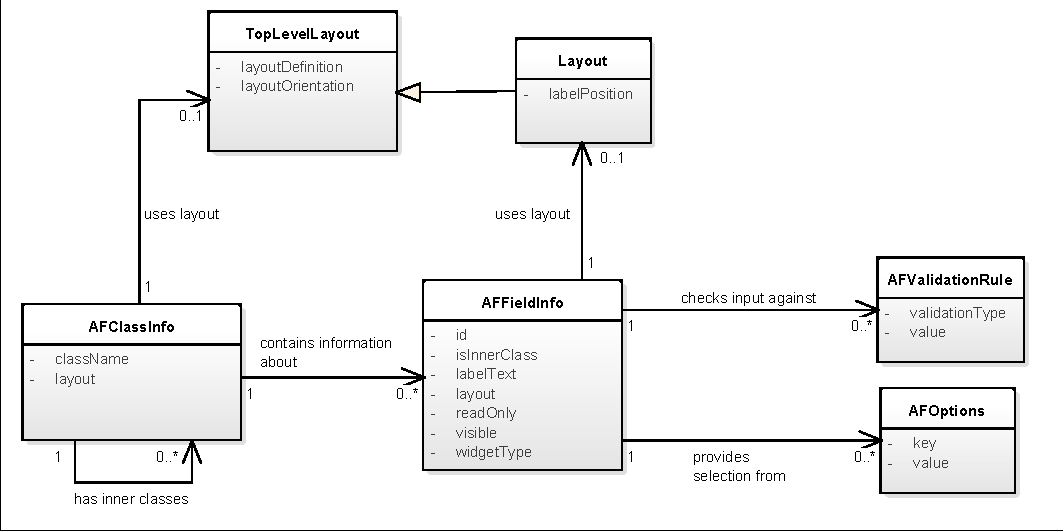
\includegraphics[width=\textwidth, trim=1 1 1 1, clip]{figures/domainModel}
\caption{Doménový model objektů obsahující metadata o komponentě}
\label{img:metadataModel}
\end{figure}

Následující část práce podrobněji rozebírá diagram z obrázku \ref{img:metadataModel}, neboť je pro vývoj obou frameworků důležitý. Android framework tuto část AFSwinx a AFRest recykluje a Windows Phone ji transformuje do jazyku C\#.
\subsubsection{AFClassInfo}
AFClassInfo udržuje informace o hlavním objektu metadat \cite{tomasek-thesis}. Obsahuje informace o názvu objektu a rozložení komponenty. Dále drží definice 0 až N informací o polích, která se mají v komponentě vyskytnout. Součástí je také 0 až N vnitřích tříd, tedy referencí na objekt stejného typu AFClassInfo. Může se totiž stát, že model, nad kterým je prováděna inspekce a ze kterého se metadata vytvářejí, obsahuje neprimitivní datový typ. Například v modelu Osoba to může být objekt typu Adresa, který obsahuje další atributy, jako třeba název ulice či město. Tento typ je ale nutno v komponentě reprezentovat také, a tak je zevnitř provedena jeho inspekce, která je později v metadatech reprezentována jako vnitřní třída. 

\subsubsection{AFFieldInfo}
Tento objekt popisuje jednu proměnnou, nad kterou byla provedena inspekce a ze které se má vytvořit pole, které se v komponentě vyskytne \cite{tomasek-thesis}. Nese informaci o widgetu, který má být při vytváření pole použit, určuje jednoznačný identifikátor pole v rámci komponenty. Dále určuje, zda má být tvořené pole viditelné a upravitelné, respektive jen pro čtení. Definuje, jak je pole rozloženo, hlavně z hlediska pozice labelu, jehož hodnota je ve AFFieldInfo rovněž zaznamenána. V neposlední řadě jsou v tomto objektu uloženy informace o validační pravidlech, oproti kterým se má validovat uživatelský vstup. Navíc v případě, že by uživatel měl mít na výběr pouze z určitých předem definovaných možností, zahrnuje AFFieldInfo i informace o těchto možnostech. 

V tomto objektu je také uloženo, zda se jedná o vnitřní třídu \cite{tomasek-thesis}, která je popsána výše. Tento fakt je velmi důležitý, neboť záleží na pořadí polí v komponentě, ve kterém mají být vykreslovány. Inspekce modelu na serveru s tím počítá, a tak pole umístí na správné místo v metadatech a označí ho jako classType, tedy vnitřní třídu, jejíž popis můžeme nalézt v metadatech v části s vnitřními třídami. V rámci zachování správného pořadí vykreslení polí je tedy nutné, aby klienstký framework fakt, že se jedná o složený datový typ, při vytváření polí komponenty zaznamenal a na pozici, kde tuto skutečnost objeví, vložil pole, o nichž jsou informace uloženy v příslušné vnitřní třídě.

\subsubsection{AFValidationRule}
Tento objekt popisuje pravidlo, které má splňovat uživatelský vstup ve vytvářeném poli \cite{tomasek-thesis}. Obsahuje typ validace, který určuje o jakou validaci se jedná a případně hodnotu pravidla. Referenční framework AFSwinx obsahuje výčtový typ s názvy validací, které podporuje a které se mohou tedy v metadatech objevit. Například definuje validační pravidlo typu MAX a hodnotou je číslo. Tedy popisuje, že hodnota v poli nesmí přesáhnout číslo určené hodnotou pravidla. 

Každé validační pravidlo má mít příslušný validátor. Ten při validaci polí komponenty provede kontrolu uživatelského vstupu podle daného pravidla a informuje framework o výsledcích. Ten musí disponovat funkcionalitou, která umožní zobrazit případné chybové hlášky uživateli. 

\subsubsection{AFOptions}
Pro určité typy widgetů, které mají být použity pro vytvoření polí, je nutné specifikovat možnosti, ze kterých si může uživatel vybírat \cite{tomasek-thesis}. Takovými widgety jsou například dropdown menu nebo skupina radio buttonů. Tento objekt popisuje tyto možnosti formou klíče a hodnoty. Klíč framework odesílá na server a hodnotu zobrazuje klientovi.

\subsubsection{TopLevelLayout}
Objekt je využit k popisu rozložení celé komponenty \cite{tomasek-thesis}. Objekt definuje dvě vlastnosti. Za prvé je to orientace, tedy ve směru jaké osy je komponenta či její část vykreslována. Dále je to definice rozložení, která má určovat, jestli je komponenta či její části vykreslovány v jednom či více sloupcích. 

\subsubsection{Layout}
Popisuje rozložení částí komponenty, tedy vytvářených polí \cite{tomasek-thesis}. Jak je patrné z obrázku \ref{img:metadataModel}, Layout dědí z TopLevelLayoutu orientaci a definici rozložení, které jsou popsány výše. Navíc má vlastnost LabelPosition, která je tvořenými frameworky využita k umístění labelu vzhledem k vytvářenému poli.

\subsection{Tvorba komponent}
Z přijatých a uložených metadat umí frameworky vytvořit dva typy komponent. Jednou komponentou je formulář, který řeší hlavně uživatelský vstup, ale může být využit, pokud je předvyplněn daty, i ke zobrazení informací uživateli. Druhou komponentou je list, neboli seznam položek, který uživateli umožňuje přehledné zobrazení většího množství informací. Ve frameworku AFSwinx tuto možnost zajišťovala tabulka \cite{tomasek-thesis}, která však není pro mobilní zařízení úplně vhodným způsobem, protože vyžaduje pro rozumné zobrazení mnoho místa, které na mobilních zařízeních zpravidla není k dispozici.

Strukturu metadat získaných ze serveru, je možné využít zároveň pro formulář i list, neboť se liší pouze grafická reprezentace metadat. Zatímco ve formuláři lze využít definic proměnných, nad kterými byla provedena inspekce, k tvorbě formulářových polí, v listu je lze použít k tvorbě informací o jedné z jeho položek. Rozložení, které je definováno ve výše popsaném TopLevelLayoutu, lze použít v případě formuláře k určení uspořádání polí. Obdobným způsobem to lze udělat v listu s uspořádáním informací o položce. List nevyužívá všechny informace, jako například typ widgetu nebo validace, ale stále je výhodnější část informací z definice nepoužít, než aby obě komponenty měly vlastní strukturu metadat. 

Pro zobrazení procesu tvorby formuláře, který je tou složitější komponentou, jelikož uživatelský vstup, který je do něj zadáván, se musí validovat a odesílat na server, narozdíl od listu, který je pouze pro čtení, byl využit diagram aktivit. Diagramy aktivit popsují určitý proces složený z dílčích podprocesů a mohou být použity například právě pro analýzu a popis algoritmu \cite{UmlArlow}. 

Z diagramu \ref{img:createFormActivityDiagram} lze odvodit, že pokud chce uživatel frameworku vytvořit formulář, musí nejdříve specifikovat, kde framework nalezne metadata. Ten o tato data požádá server. Server musí samozřejmě data dynamicky vytvořit, a tak provede inspekci, která byla zmíněna výše, a vytvoří metadata, která klientskému frameworku předá zpět. Ten je zpracuje a vytvoří na základě nich požadovanou komponentu. Pokud uživatel zároveň nadefinoval i zdroj dat, kterými by se měl formulář naplnit, požádá klient znovu server o tato data. Server je vygeneruje a zašle zpět, načež se komponenta těmito daty naplní. Poté se takto vytvořená komponenta předá uživateli, tedy vývojáři, který s ní může dále pracovat, například ji vložit do GUI tam, kam potřebuje.

Navržená struktura frameworku sloužící k realizaci procesu tvorby komponenty je zobrazena v části doménového modelu systému na obrázku \ref{img:domainModelBuild}. Strukturu na obrázku následující část práce blíže specifikuje.

\begin{figure}[h!]
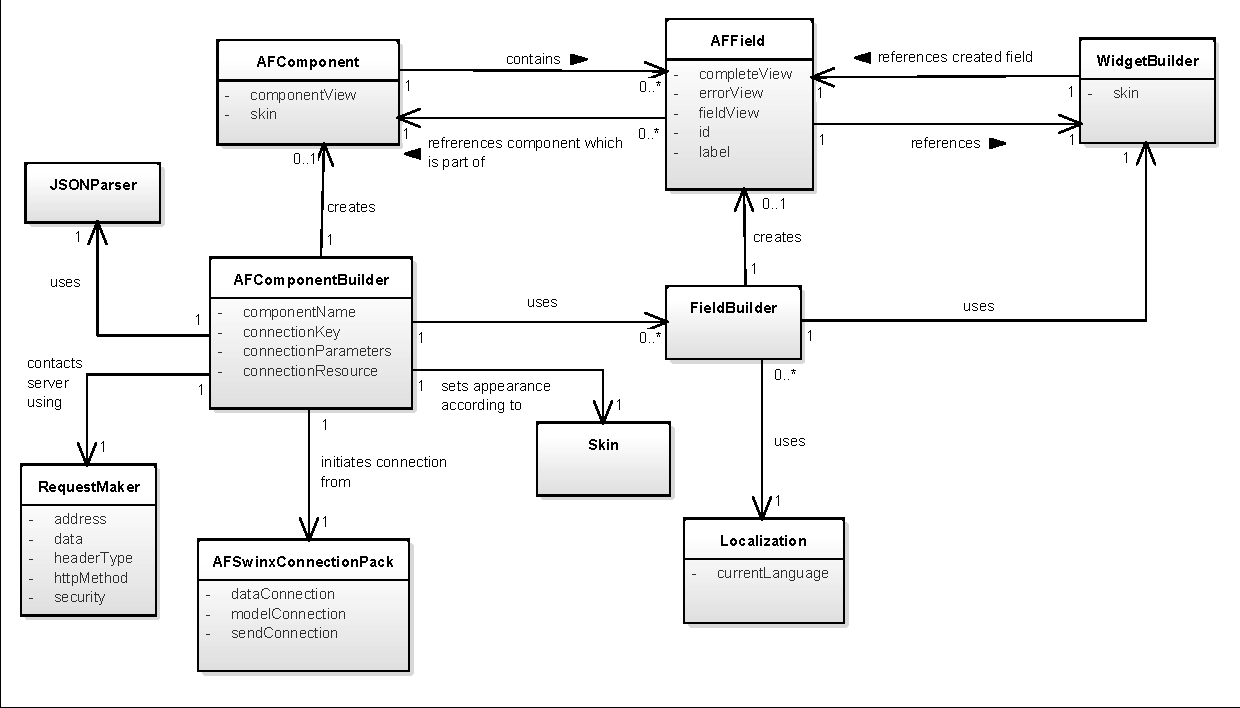
\includegraphics[width=\textwidth, trim=1 1 1 1, clip]{figures/domainModelBuild}
\caption{Část doménového modelu systému realizující tvorbu komponenty}
\label{img:domainModelBuild}
\end{figure}

\subsubsection{AFComponent}
Tato třída zastřešuje vytvořenou komponentu. Jak bylo již zmíněno, frameworky podporují dva typy komponent, a to formulář a list. Grafická reprezentace komponenty je uložena v atributu componentView. Také obsahuje skin, podle kterého je vzhled komponenty nastaven. Komponenta obsahuje 0 až N tříd typu AFField, které jsou popsány v následující sekci.

\subsubsection{AFField}
AFField popisuje vytvořenou část komponenty, tedy její pole. Pole má svůj jednoznačný identifikátor a je složeno ze tří grafických prvků. Prvním prvkem uloženým v atributu fieldView je widget, kterým je pole v GUI reprezentováno. Druhým prvkem je errorView, který slouží pro zobrazení validačních chyb uživateli, a posledním prvkem je label neboli popisek pole. Všechny tři prvky se kombinují v daném rozložení do atributu completeView, který v první řadě poskytuje jednoduchý přístup k celkové grafické reprezentaci pole.

\subsubsection{AFComponentBuilder}
Pro rozlišení, zda se z metadat vytvoří formulář nebo list, jsou vytvořeny dva typy builderů, které komponenty staví. Uživateli, který framework používá, tedy stačí specifikovat builder, který požadovanou komponentu vytvoří. Aby bylo používání frameworků co nejvíce uživatelsky přívětivé, způsoby tvoření builderů a jejich používání by se neměly lišit. Uživateli stačí naučit se pouze vytvořit jeden typ komponenty a druhý typ vytvoří pouze výměnou builderu. Na obrázku \ref{img:domainModelBuild} jsou buildery vyobrazeny jako AFComponentBuilder. Z digramu je patrné, že může builder vytvářet 0 až 1 komponent, to znamená, že builder může být pouze nadefinován a nemusí být použitý pro tvorbu komponenty, čímž však ztrácí svůj smysl, proto případ tvorby žádné komponenty s největší pravděpodobností nenastane, nicméně je možný. Uživatel při specifikaci builderu může nastavit jednoznačný identifikátor komponenty, kterou tvoří, což reprezentuje atribut componentName. Dále je nutné určit již zmíněný XML soubor s definicemi připojení, který reprezentuje atribut connectionResource. V tomto souboru se vybere příslušné připojení na základě uživatelem zadaného klíče v atributu connectionKey. Atribut connectionParameters definuje dodatečné parametry ve formě klíč-hodnota pro připojení na server. Takovými parametry mohou být například uživatelské jméno a heslo sloužící pro autorizaci uživatele, kterému se má komponenta zobrazit. Na základě těchto specifikací se ze zmíněného XML souboru \ref{code:xmlSource} vytvoří připojení pro definici komponenty, data a odeslání dat z komponenty na server, která se uloží do třídy AFSwinxConnectionPack, která je součástí referenčních frameworků AFSwinx a AFRest \cite{tomasek-thesis}.

\subsubsection{RequestMaker a JSONParser}
Definovaných připojení využije třída RequestMaker, zajišťující komunikaci builderu se serverem. Tato třída vytváří HTTP requesty na URL adresu definovanou v atributu address. Použije k tomu metodu specifikovanou v httpMethod. Možné metody jsou get, post, put, delete. Atribut data obsahuje případná data, která se mají na server odeslat, atribut headerType určuje formát těchto dat. Zdroje mohou být zabezpečené, proto je zde i atribut security, který definuje uživatele a bezpečnostní metodu. Prozatím je podporována pouze BASIC autentifikace.

Pokud se třída využije pro zisk definice komponenty, následuje, jak již bylo zmíněno, rozbor této definice a její následné umístění do struktury pro uložení metadat, která byla popsána na obrázku \ref{img:metadataModel}. K tomuto účelu AFComponentBuilder využívá dle obrázku \ref{img:domainModelBuild} třídu JSONParser. 

\subsubsection{FieldBuilder a WidgetBuilder}
Komponenta se skládá z několika částí, tedy polí komponenty, které je potřeba také vytvořit. O to se stará FieldBuilder, který vytváří žádné nebo jedno pole. Podobně jako u AFComponentBuilder je případ nevytvoření pole velmi nepravděpodobný, protože by builder ztratil svůj účel. FieldBuilder slouží pro vytvoření tří prvků GUI, které pole obsahuje, jak bylo popsáno u AFField. 

K vytvoření části, která určuje widget komponenty se využívá WidgetBuilder. V metadatech se nachází pro každé pole, které má být součástí komponenty, typ widgetu, kterým má být pole reprezentováno. Například to může být textové pole, checkbox nebo skupina radio buttonů. Ke každému widgetu existuje vlastní builder, reprezentovaný právě touto třídou. WidgetBuilder nejen widget vytváří, ale také určuje, jak se z widgetu dají získat data a naopak, jak je do něj vložit. WidgetBuilderu je také předáván skin, který určuje, jak widget vypadá.

\subsubsection{Lokalizace}
V rámci metadat, která přijdou ze serveru se mohou objevit texty určené pro lokalizaci, tedy překlad. Tyto texty jsou realizované pomocí klíčů, ke kterým lze překlad přiřadit a vyskytují se v labelech, v možnostech, ze kterých může uživatel v daných typech widgetů vybírat, nebo ve validačních chybách. Frameworky tedy musí disponovat funkcionalitou, který tuto lokalizaci umožní včetně změny jazyka za běhu aplikace. K tomu FieldBuilder používá třídu Localization, která má atribut currentLanguage zachycující aktuální jazyk. Aby byl způsob lokalizace textů v aplikaci jednotný, je možné využít lokalizační část frameworku i nad jeho rámec například k překladu textů tlačítek či položek v menu. 

\subsection{Práce s vytvořenou komponentou}
Komponentu nestačí jen vytvořit, ale cílem frameworku je také umožnit s ní další práci. Vývojáři by mělo být umožněno například odeslat formulář, zkontrolovat to, co uživatel zadal, nebo upravit vzhled komponenty. Práci s komponentou lze demostrovat na práci s formulářem. Pro tento účel byl vytvořen diagram aktivit, který popisuje tři hlavní možnosti práce s formulářem a to odesílání dat, resetování a vyčištění formuláře. Tento diagram lze nalézt v příloze \ref{img:formWorkActivityDiagram}.

V případě odesílání dat diagram popisuje, že se data nejdříve musí validovat. Pokud data nejsou validní, zobrazí se validační chyby a proces končí. Pokud však validní jsou, hraje roli ještě fakt, zda je nebo není nadefinovaný zdroj, kam se data mají odeslat. Pokud zdroj chybí, je o tomto informován uživatel a proces znovu končí. Pokud zdroj nechybí a proces pokračuje dále, data se zformují do podoby, kterou server vyžaduje, a odešlou se. Jelikož jsou data validní a ve správném formátu, server nebude mít problém je přijmout a zpracovat. Výsledek zpracování je propagován vývojáři, který s ním dle svého uvážení naloží. Tím proces odeslání končí. 

Aby vývojář mohl s komponentou pracovat, musí být schopen ji získat, nejlépe kdekoliv v programu. Proto se vytvořené komponenty musí někde skladovat a být k nim jedoduchý přístup. V případě Androidu je pro tento účel navržena třída AFAndroid, v případě Windows Phone třída AFWinPhone. Tyto třídy nabízí mimo získání komponent i možnost vytvoření obou typů builderů a uživateli tak zprostředkovává vlastně vše, co pro vytváření komponent potřebuje.

\section{Případy užití}
V této sekci se práce zaměřuje na případy užití, které zachycují návrh možností, které by měly oba mobilní frameworky podporovat. Ke zobrazení těchto možností slouží diagram případů užití, který lze nálezt v příloze \ref{img:useCaseModel}. Případy užití určují, jak lze používat systém nebo jeho dílčí části \cite{UmlArlow}. Případ užití je iniciován aktérem, jímž je v tomto případě hlavně vývojář, který framework používá. V této práci je část případů užití definována i pro samotný framework, která zobrazuje, jaké akce musí framework provést pro splnění úkolu zadaným uživatelem. Definici posloupností jednotlivých akcí popisuje vždy příslušný scénář případu užití. 

Jednou z hlavních funkcí, kterou musí frameworky podporovat, je odeslání formuláře. Tato funkce je blíže popsána obrázkem \ref{img:useCaseModelFormSend}, na kterém jsou zobrazeny potřebné případy užití \cite{tomasek-thesis}. Tento obrázek je podrobněji přiblížen popisem a scénářem každého případu užití, který se v něm vyskytuje. Pro stručnost je předpokládán hladký průběh scénáře, samozřejmě všude tam, kde se vyskytne IF, tedy podmínka, by měl být uveden i alternativní scénář, který řeší to, co se stane při nesplnění podmínky.

\begin{figure}[h!]
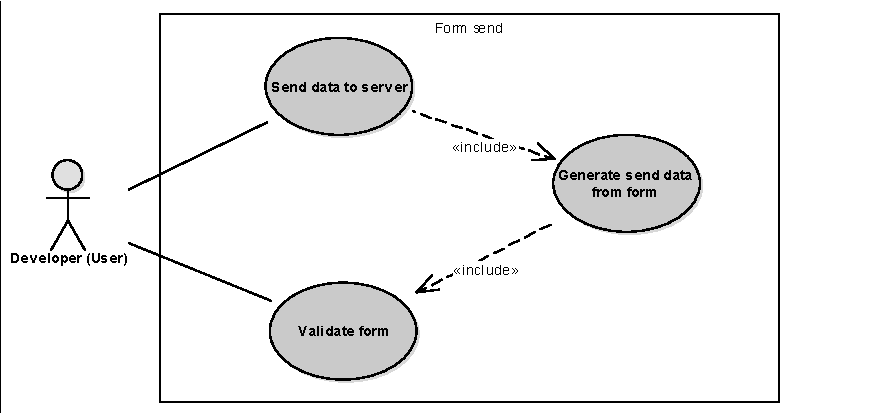
\includegraphics[width=\textwidth, trim=4 4 4 4, clip]{figures/useCaseFormSend}
\caption{Část diagramu případů užití pro odeslání formuláře}
\label{img:useCaseModelFormSend}
\end{figure}

\subsection{Případ užití: Validace formuláře}
Na obrázku \ref{img:useCaseModelFormSend} se tento případ jmenuje Validate form a má zachycovat validaci uživatelského vstupu ve formuláři. Z diagramu také vyplývá, že by uživatel měl být schopen užívat validaci formuláře i explicitně, tedy ne jen v rámci odeslání dat. Následující scénář tohoto případu užití popisuje postup, jak by měla validace formuláře probíhat.\\\\
Vstupní podmínky:
\begin{itemize}
\item Framework zná formulář, který chce validovat. 
\item Tento formulář musí být vytvořený za pomoci metadat.
\end{itemize}
Scénář případu užití:
\begin{enumerate}
\item Uživatel požádá systém o validaci daného formuláře.
\item Systém získá z formuláře všechna pole.
\item WHILE existuje nezvalidované pole DO
\begin{enumerate}
\item Systém získá všechna pravidla, kterým pole podléhá.
\item WHILE existuje nenavštívené pravidlo DO
\begin{enumerate}
\item Systém získá pro dané pole a pravidlo příslušný validátor.
\item Systém provede validaci.
\item IF validace selhala THEN
\begin{enumerate}
\item Systém přidá k chybovým hláškám určeným pro zobrazení příslušnou hlášku o chybě validace.
\end{enumerate}
\end{enumerate}
\item IF alespoň jedna z validací na poli selhala THEN
\begin{enumerate}
\item Systém zobrazí k danému poli validační chyby.
\end{enumerate}
\end{enumerate} 
\end{enumerate}

\subsection{Případ užití: Vygenerování odesílaných dat}
Tento případ užití popisuje akci frameworku, která musí být provedena, aby šlo úspěšně na server odeslat data. Framework nezná přímo objekt, který chce na serveru odesláním dat vytvořit nebo upravit. Co však zná, je jeho struktura, na základě které samotný objekt nevytvoří, ale je schopen poskládat pro server přijatelná data. Z těchto dat si server, který objekt již zná, dokáže tento objekt vytvořit. Důležitý je formát dat, ve kterém mají být serveru tato data zaslána. Referenční AFSwinx a AFRest podporují prozatím jen JSON formát, ale počítá se s přidáním dalších formátů \cite{tomasek-thesis}. Bylo by tedy dobré, navrhnout tento případ užití pro více možných formátů. V diagramu \ref{img:useCaseModelFormSend} je tento use case nazván Generate send data from form a popisuje ho níže zmíněný scénář.\\\\
Vstupní podmínky:
\begin{itemize}
\item Framework zná formulář, ze kterého chce sestavovat data pro odeslání. 
\item Tento formulář musí být vytvořený za pomoci metadat. 
\item Framework musí znát serverem akceptovaný formát dat. 
\end{itemize}
Scénář případu užití:
\begin{enumerate}
\item Uživatel chce sestavit z formuláře data k odeslání.
\item <<include>> Validovat formulář
\item IF validace proběhla úspěšně THEN
\begin{enumerate}
\item Systém získá z formuláře všechna pole.
\item WHILE existuje pole, které nebylo zahrnuto v odesílaných datech DO
\begin{enumerate}
\item Systém získá builder, který pole postavil.
\item Systém požádá builder o data, která se v poli nacházejí.
\item  Systém určí název proměnné a třídu, do které patří, a nastaví jí data.
\item  Systém podle formátu dat, které server očekává, rozhodne, v jakém formátu data zaslat a na tento formát data převede. 
\end{enumerate}
\end{enumerate}
\end{enumerate}

\subsection{Případ užití: Odeslání dat na server}
Posledním případem užití z obrázku \ref{img:useCaseModelFormSend} je use case Send data to server. Ten zahrnuje předchozí případ, což je popsáno v níže uvedeném scénáři.\\\\
Vstupní podmínky:
\begin{itemize}
\item Framework zná formulář, ze kterého chce sestavovat data pro odeslání.
\item Tento formulář musí být vytovřený za pomoci metadat.
\item Framework musí znát zdroj, na který mají být data odeslána, a všechny potřebné informace, které zdroj vyžaduje. 
\end{itemize}
Scénář případu užití:
\begin{enumerate}
\item Uživatel chce odeslat data z formuláře na server.
\item <<include>> Vygenerování odesílaných dat
\item IF bylo vytvoření dat z formuláře úspěšné THEN	 
\begin{enumerate}
\item Systém odešle data na specifikovaný zdroj.
\item Systém informuje uživatele o výsledku akce.
\end{enumerate}
\end{enumerate}

\subsection{Úprava vzhledu komponenty}
Důležitým aspektem grafického uživatelského rozhraní je také jeho vzhled, neboť špatně navržený vzhled GUI může vést i k ohrožení použitelnosti aplikace. V Android aplikacích se vzhled definuje buď v XML šablonách pro daný view, to v případě, že je GUI vytvořeno staticky \cite{android-themes}, nebo pomocí Javy v případě dynamického přístupu. 

Na Windows Phone platformě jsou obdobou XML šablon XAML soubory, které z XML vycházejí, a případě dynamického vytváření slouží k úpravě metody napsané v C\#. Ve Windows Phone aplikacích se preferuje neměnit barvy komponent, protože ke změně barev slouží barevná témata, která mají výhodu v tom, že jsou konzistentní na všech zařízeních \cite{wp-themes}, ale ovlivňují mimo GUI operačního systému také GUI aplikací. Může se tedy stát, že pokud vývojář nastaví například barvu textu na bílou a aktuální téma, které zařízení používá, má bílé pozadí, nebudou texty jednoduše viditelné. Windows Phone verze frameworku tedy musí zohlednit i tyto situace.  

Jelikož se komponenty tvoří dynamicky v rámci frameworku a uživatel k procesu tvorby nemá explicitně přístup, je nutné poskytnout mu možnost nadefinovat vzhled komponenty předem. K tomuto účelu frameworky disponují skiny, které má uživatel možnost nastavit builderu komponenty. V příloze \ref{img:useCaseModel} se tento případ užití nazývá Nastavit skin. V případě, že by uživatel frameworku skin nenadefinoval, existuje základní vzhled. Od tohoto základního skinu může uživatel ve svých skinech dědit a překrýt pouze části, které mu nevyhovují a chtěl by je změnit. Po sestavení komponenty už není jednoduše možné za pomoci frameworku tento vzhled změnit. I když framework poskytuje možnost získat grafickou reprezentaci komponent i jejich částí, změna vzhledu těchto částí vyžaduje znalost dynamické tvorby UI na jednotlivých platformách.

\subsection{Životní cyklus formuláře}

Komponenty přecházejí během svého života mezi různými stavy neboli mají svůj životní cyklus, který lze popsat pomocí diagramu stavů \cite{UmlArlow}. Na obrázku \ref{img:formStateDiagram} je popsán životní cyklus formuláře \cite{tomasek-thesis}. Formulář se nachází v inicializačním stavu, na obrázku \ref{img:formStateDiagram} označen jako Initialized, pokud už byl vytvořen a případně naplněn daty. Komponenta přejde do stavu Inconsistent, pokud data, kterými je komponenta naplněna, nesplňují definovaná validační pravidla. To může nastat ve dvou případech. Prvním je, že se komponenta již nevalidními daty naplní v průběhu tvorby, druhým případem je, že nevalidnost dat způsobí uživatel jejich úpravou, čemuž na obrázku \ref{img:formStateDiagram} odpovídá přechod ze stavu Modified, který je popsán dále, do stavu Inconsistent. Komponenta setrvává ve stavu Inconsistent, pokud uživatel data nezmění a opakovaně provádí validaci končící neúspěchem. Stav Modified značí, že data v komponentě byla modifikována. Dokud je komponenta upravována, setrvává v tomto stavu. Do stavu Modified se komponenta může dostat ze stavu Initialized, Inconsistent a Synchronized. V případě provedení úspěšné validace přechází z tohoto stavu komponenta do stavu Consistent, který značí, že je komponenta připravená na odeslání na server. Odeslání může být neúspěšné, v tom případě se komponenta stává nekonzistentní, nebo úspěšné, čímž přejde do stavu Synchronized. Odtud může přejít do stavu Modified, pokud jsou data modifikována, nebo do inicializačního stavu, pokud byla data v komponentě aktualizována opětovným načtením ze serveru \cite{tomasek-thesis}.

\begin{figure}[h!]
\centering
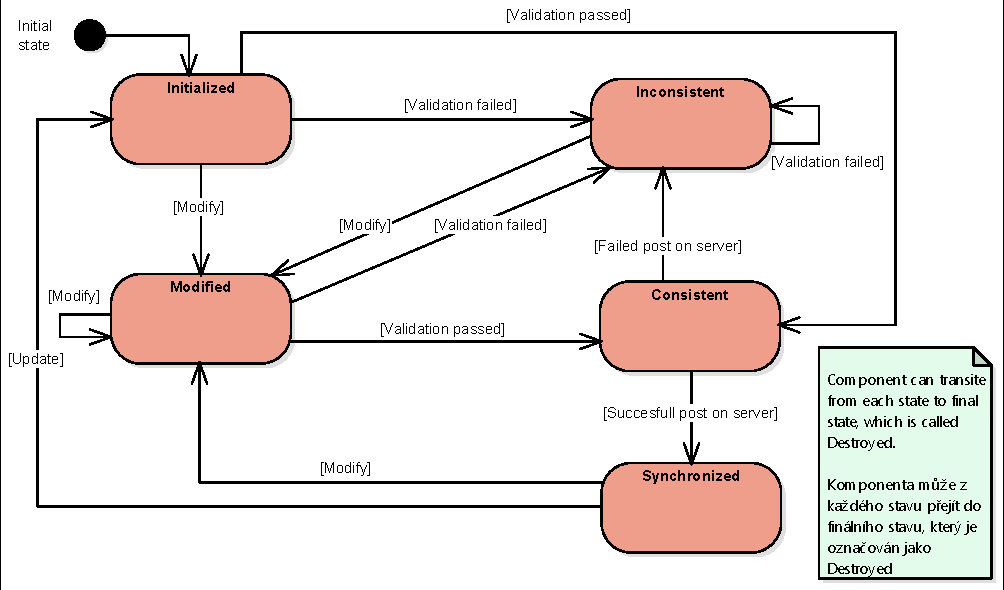
\includegraphics[width=0.87\linewidth, trim=1 1 1 1, clip]{figures/stateDiagram}
\caption{Diagram stavů popisující životní cyklus formuláře}
\label{img:formStateDiagram}
\end{figure}

\section{Práce na existujícím řešení}
Cílem práce je také rozšířit stávající verzi frameworků AFSwinx a AFRest. Pro tento účel bylo rozhodnuto přidat novou anotaci, kterou zohlední dříve zmiňovaná inspekce na serveru při tvorbě metadat. Cílem anotace je sdělit klientovi, že se má anotací označený atribut v modelu na serveru porovnat s druhým atributem, který je určen v parametrech anotace, ve smyslu menší nebo rovno než. Anotace se týká hlavně atributů typu datum a řeší, zda tento atribut obsahuje datum dřívejší nebo stejné než druhý atribut určený v parametrech anotace. Anotace má tedy funkci validačního pravidla. Tato informace se v metadatech objevuje prozatím pouze u informací o poli s typem widgetu, jenž má být reprezentován jako datepicker. AspectFaces \cite{aspect-faces} ve své dokumentaci popisuje, že pokud chce uživatel přidat novou anotaci, musí vytvořit tzv. anotační deskriptor, který musí zaregistrovat v konfiguračním souboru aspectfaces-config.xml uloženém ve složce WEB-INF. Tím se zajistí, že inspekce anotaci promítne do metadat ve formě XML. AFSwinx a AFRest tyto XML soubory poté převádí do platformově nezávislé podoby \cite{tomasek-thesis} a v tomto procesu je nutné taktéž provést změny. Po vytvoření anotace je nutné přidat ji na daná místa na serveru a je žádoucí vytvořit validátory nejen v obou vytvářených frameworcích pro mobilní platformy, ale také v již existujícím řešení AFSwinx pro platformu Java SE.

\section{Použité technologie}
V této části práce jsou popsány použité technologie. Kromě samotných frameworků jsou součástí práce i příslušné ukázkové projekty.

\subsection{Java a Android SDK}
Část frameworku, která je schopná vytvářet formuláře nebo listy pro Android aplikace a poté s nimi pracovat, k tomu využívá právě těchto dvou technologií. Zdrojové kódy Android aplikací jsou psány v Javě a ty se přeloží pomocí Android SDK do APK souboru spustitelném na mobilním zařízení. Android SDK poskytuje Java knihovny pro dynamické vytváření prvků UI jako jsou komponenty, layouty, dialogy, posluchače akcí atp. Také poskytuje širokou škálu funkcí k práci se souborovým systémem, senzory, sítí, kamerou a mnoho dalších funkcí \cite{android-intro}. Android je na spoustě různorodých zařízeních a vyskytuje se v mnoha různých verzích, proto je třeba zvážit, na jaká zařízení je aplikace mířena. Obecně platí, že čím nižší verze SDK, tím méně poskytovaných funkcí. Při vytváření projektu v IDE Android Studio se vývojář dozví, že pokryje 100\% zařízení, pokud cílí svůj projekt alespoň na verzi 10, která odpovídá Android verzi 2.3.3 nebo 2.3.4. s kódem Gingerbread z února 2011 \cite{android-sdks}. Framework AFAndroid je nastaven na podporu SDK verze 11, neboť využívá pro kontaktování serveru třídu AsyncTask, která je dostupná až od této verze. Nicméně framework byl otestován kvůli absenci staršího zařízení až na SDK 18, tedy verzi Android 4.3.3 s kódem Jellybean \cite{android-sdks}, na kterém framework funguje bezchybně. Při vývoji této části frameworku bylo využito IDE Android Studio 1.5.1.

\subsection{C\# a Windows Phone SDK}
Další část práce se věnuje Windows Phone verzi frameworku. Aplikace na Windows Phone je obvykle psaná v jazyce C\# \cite{wp-csharp} za pomoci knihoven z Windows Phone SDK, které obdobně jako Android SDK umožňují dynamické tvoření UI, reagovat na vzniklé události, pracovat s mobilním zařízením atd. Ačkoliv není Windows Phone tolik rozšířen jako Android, taktéž existuje více verzí operačního systému, mezi kterými je potřeba se rozhodnout. Tato práce se zaměřuje na Windows Phone 8.1, protože dle statistik z března 2016 je nejpoužívanější Windows Phone verzí a starších verzí ubývá. Naopak přibývájí uživatelé novější verze Windows 10 Mobile, která by ale neměla mít problém aplikace pro starší telefony spustit \cite{wp-statistics}. Při vývoji WP části frameworku bylo využito vývojové prostředí Visual Studio 2015 od společnosti Microsoft.

\subsection{AFSwinx a AFRest}
AFSwinx a AFRest \cite{tomasek-thesis}, které byly již dříve popsány v sekci s existujícími řešeními, jsou napsány v Javě. Jsou k dispozici v podobě JAR souborů, které Android verze frameworku importuje a využívá. Windows Phone verze je použít nemůže, neboť se liší platformou, a vše, co bylo Android frameworkem využito, musí být do WP přepsáno.
Použité části těchto frameworků byly popsány v dřívějších částech této kapitoly, jako například struktura pro uložení metadat na obrázku \ref{img:metadataModel}.

\subsection{Ukázkové projekty}  
Ukázkové projekty demostrují použití obou vytvořených frameworků. Pro splnění tohoto úkolu bylo zapotřebí také následujících technologií.
\subsubsection{AFServer}
Jak bylo již zmíněno, oba frameworky AFAndroid i AFWinPhone interpretují určitý popis uživatelského rozhraní, který přichází ze serveru, který takový popis dokáže poskytnout. Tento server byl již vytvořen pro demostraci funkčnosti frameworků AFSwinx a AFRest a je využit i pro ukázkové projekty v této práci. AFServer je Java EE aplikace, která využívá technologií jako RestEasy, která poskytuje API pro definici RESTful webových služeb, nebo například in-memory databázi DerbyDB \cite{tomasek-thesis}. 
\subsubsection{Glassfish}
Glassfish \cite{glassfish} je open-source aplikační server využívaný pro Java EE platformu. Zmiňovaný AFServer je odladěn pro použití právě na Glassfish ve verzi 3 a 4, a proto, když bylo potřeba server při vývoji ukázkových projektů použít, byl spuštěn přes tento aplikační server \cite{tomasek-thesis}. Server byl spouštěn při vývoji ukázkových projektů lokálně. Později byl server umístěn na doménu \url{www.toms-cz.com/AFServer}, aby mohl být testován i z mobilních zařízení a ne pouze pomocí emulátorů. Pak již nebylo potřeba explicitně Glassfish používat.
